Individuals who have few resources can join together to achieve common goals
by engaging in collective action.
However, to achieve their goals, those individuals must be able to collaborate
effectively.
Collaboration requires both that individuals can agree on which actions they
should take, and that they can coordinate those actions effectively.
Both collective decision-making and coordination
have been studied in the in the context of collective intelligence.
This chapter reviews work on both collective action and collective intelligence,
and discusses how the latter can inform the former.

No unified theory or framework of collective action exists (Ostrom, 2000).
For the purpose of this review,
I will adopt a framework consisting of four stages: ideation, deliberation,
decision-making, and execution (Figure \ref{fig:framework}).
These stages are roughly sequential, but occur simultaneously in varying combinations
over the course of actual collective action.
The ideation stage consists of generating ideas for possible actions,
as occurs in commons-based peer production.
Deliberation consists of discussing problems and proposed solutions,
as occurs in social learning and the discourse of the public sphere.
In decision-making, group members aggregate their individual preferences into
a social preference for the entire group, as formalized in social choice theory.
Finally, in the execution stage, once a decision has been agreed on, group members act,
either complying with the group's decision or, if some dissent and conflict remain, defecting.

\section{Collective Action}
Much of the existing literature on collective action focuses on two questions.
First, what are the conditions that lead to cooperation? And second, when is cooperation effective?

\subsection{Cooperation}
Collective action depends on the cooperation of group members, including contributions of resources. Olson's zero contribution thesis argues that cooperation in public goods settings is only possible in small groups or through coercion (Olson, 1965). When individuals can free-ride on the contributions of others without fear of punishment, the situation resembles a multiplayer prisoner's dilemma.
A rational egoist has an equilibrium solution of zero contribution
and should never cooperate willingly.
But willing cooperation does sometimes occur in the world. Experiments show that people often behave as {\em conditional cooperators},
and {\em willing punishers} (Ostrom, 2000). Conditional cooperators are trusting when they expect that trust to be reciprocated. Willing punishers choose to punish norm violations even when the costs outweigh the benefits.

Why does cooperation occur? Real individuals are not always motivated by rational egoism. As Yochai Benkler writes, ``there exist ranges of human experience in which the presence of monetary rewards is inversely related to the presence of other, social-psychological rewards (2002).'' He cites examples including marriage, sex, and gift exchange. Ostrom (2000) proposes that the human deontic problem-solving system (reasoning about norms, guilt, and shame) has enabled us to adopt cooperative behaviors despite their apparent short-term irrationality. Ironically, these behaviors may be more rational than they seem when taking a long-term, large-scale perspective. In evolutionary models of a repeated prisoner's dilemma, communities of trusting individuals can outperform less trusting individuals (Axelrod, 1997a). Ostrom suggests that the deontic problem-solving system allows members of a society to learn seemingly irrational cultural norms such as trust, when those norms allow the society to thrive in the long run.

\subsection{Collaboration}
While collaboration allows groups to apply their resources to problems that individuals
cannot solve on their own, some of those resources must be spent on communication and coordination, contributing to {\em process loss} (Steiner, 1972),
possibly limiting the usefulness of collaboration. Both organizational psychologists and economists have investigated when the benefits of collaboration outweigh the costs.

In a review of organizational psychology research, Hill (1982) concluded that groups typically performed better than individuals, while taking longer to find a solution. However, except in a few cases, statistical aggregates or high skilled individuals performed at least as well as groups. Exceptions were for difficult and complex tasks like crossword puzzles which no individual could solve on their own,
as has also been seen in agent-based and theoretical results (Hong \& Page, 2004).
Hill attributed benefits of group work to process gain from social learning (see Section \ref{sec:social-learning}),
but concluded that talented individuals will often out-perform committees when those committees have low-performing individuals.
However, this conclusion ignores that difficult, complex problems may be a more realistic and more important scenario.

Informed by case studies of shared resources such as municipal water supplies, police departments, forests, and fisheries, Elinor Ostrom (2000; 2010) proposed the following set of design patterns for long-surviving, self-organized common pool resource governance regimes.
\begin{description}
\item[Boundaries.]{Clear boundaries delineating who is and is not a member of a group enable the development of within-group reciprocity and trust.}
\item[Rules for appropriation and provision.]{Rules reduce uncertainty by defining required contributions of inputs and the conditions for resource use. Rules are congruent with local conditions. Such rules are not necessarily formal.}
\item[Collective Choice Arrangements.]{When all individuals affected by rules are able to participate in creating them, rules are both better adapted to local conditions and have more legitimacy in the eyes of the group.}
\item[Monitoring of Users and Resources.]{Users select individuals to monitor both resources and users (including the monitors themselves) within the regime.}
\item[Graduated Sanctions.]{Sanctions for users who violate rules and norms begin light, but become more severe with repeated misconduct. Sanctions help to publicly reinforce norms as well as the trust that they will be followed. Furthermore, sanctions allow past transgressors to demonstrate cooperation and rebuild trust.}
\item[Conflict Resolution Mechanisms.]{Conflicts over interpretations of rules inevitably arise. Fast and effective means of resolving those conflicts help maintain trust.}
\item[Minimal Recognition of Rights.]{External authorities recognize the rights of the group. Without such recognition, an appeal to authority could be used as a threat to destroy the group.}
\item[Nested Enterprises.]{When resources exist at multiple scales, they are governed by nested organizations, each adapted to a particular scale.}
\end{description}

Ostrom also identifies the following common anti-patterns that pose a threat to sustained collective action by creating unpredictability, eroding trust, or creating rules at odds with local conditions.
\begin{enumerate}
\item{Migration,}
\item{Government imposed rules,}
\item{Rapid changes in technology,}
\item{Transmission failure,}
\item{Reliance on external aid,}
\item{External aid disconnected from local knowledge and institutions,}
\item{Corruption,}
\item{Conflict between regimes.}
\end{enumerate}

\subsection{Types of Collaboration}
An analysis of a process as complex as collective action could potentially focus on any number of factors. Hill (1982) suggests a two-dimensional framework based on {\em interpersonal context} and {\em performance evaluation}. Interpersonal context describes how individuals interact. Isolated individuals have no interaction, but their outputs might be aggregated, e.g., Galton's ox (1907). Coacting individuals interact freely and synchronously, as in a typical, face-to-face meeting. Dispersed interactions occur asynchronously, as is more typical of online collaborations (Benkler, 2002). Performance can be evaluated based on each individual, the best member's output, the union of all members output (e.g., brainstorming), or a single collaborative output.

Ostrom (2000) also identified several factors that might be relevant to the functioning of a specific collective regime.
\begin{enumerate}
\item{Type of production and allocation functions,}
\item{Predictability of resource flows,}
\item{Relative scarcity of the good,}
\item{Size of the group,}
\item{Heterogeneity of the group,}
\item{Dependence of the group on the good,}
\item{Common understanding of the group,}
\item{Size of the total collective benefit,}
\item{Marginal contribution by one person to the collective good,}
\item{Size of the temptation to free ride,}
\item{Loss to cooperators when others do not cooperate,}
\item{Having a choice of participating or not,}
\item{Presence of leadership,}
\item{Past experience and level of social capital,}
\item{Autonomy to make binding rules.}
\end{enumerate}
 
So far, I have focused on collective action at a macro level. In order to understand the role of the internet in large-scale collective action, it is necessary to use a finer-grained analysis. Different stages of the collective action process (Figure \ref{fig:framework}) tend to be studied in different fields. Ideation is studied in organizational psychology, deliberation in sociology and political science, decision-making in economics and political science, and action execution in sociology, anthropology, public policy and epistemology.

This prelim focuses specifically on deliberation, so I expand my analysis of the deliberation stage to include both predictions of which actions will lead to which outcomes and individual preferences over those outcomes. Predictions can be influenced by information and reasoning, whether that information is gained through social interaction or gained through non-social means such as a search engine. Preferences can only be influenced through social, human-to-human {\em discourse} (Habermas, 1964; Geiger, 2009), for example, by creating identification with a community, emotional contagion, empathy, and so on (discourse will be described in more detail in Section \ref{sec:discourse}). For example, when friends discuss which toppings to order on a pizza, the strength of the friendship may influence which toppings they are willing to consider, but it is unlikely to influence their prediction of what will arrive if they place an order for pineapple. These two effects of deliberation are particularly important to distinguish in an online setting, where interactions can range from non-discursive to highly discursive.

\begin{figure}
\centering
\includegraphics[width=4.75in]{images/fig-framework.pdf}
\caption{
Collective action framework.\label{fig:framework}
}
\end{figure}

\section{The Economics of Peer-Production}
The internet has enabled near-instantaneous, many-to-many communication at a previously unknown scale. These affordances of the internet are promising not just for enabling larger collaborations, but because they enable collaborations that follow fundamentally different economics. Yochai Benkler (2002, 2006) labels this new form of economic production {\em commons-based peer production}, in contrast to more traditional forms of organization and production: firms, markets, and states (Coase, 1937; Ostrom, 2010). The new form is ``commons-based'' for two reasons. First, because outputs are contributed to the knowledge commons (a public good). Second, despite the non-rivalrous nature of the knowledge commons, there is incentive for free-riding and social loafing, analogous to the ``tragedy of the commons'' that occurs for common goods. The form is peer-produced because it is non-hierarchical: tasks are self-selected within a group of peers, rather than assigned from a superior to a subordinate. Benkler (2002) discusses examples including: NASA click workers, Wikipedia, the Google search engine, and the web forums Slashdot and Kuro5hin. Commons-based peer production faces the same motivational and organizational challenges as other forms of collective action, but offers both new resolutions to those challenges as well as novel advantages.

In addition to the usual motivations for non-rational-egoist behavior, commons-based peer production offers a unique solution to the problem of motivation: decomposability (Benkler, 2002). When tasks can be broken up into small pieces, each of those pieces requires smaller amounts of motivation relative to tasks performed in a traditional firm. Furthermore, when those sub-tasks can be shared with a very large group, it is easier for individuals to identify the sub-tasks best matched to their particular level and type of motivation. Decomposability makes it possible for dispersed teams to collaborate on a problem (Hill, 1982). Dispersed interactions create additional coordination challenges: accreditation (quality control) and integration of outputs (Benkler, 2002). There are many possible approaches to accreditation and integration: hierarchical, norms-based, or aggregation/averaging, for example. Or, as in the case of peer review, these tasks can also be peer-produced. Peer-production of accreditation and integration is a key component of Benkler's formulation of commons-based peer production. Using Hill's classification (1982), commons-based peer production tasks use a group product evaluation criterion. Note that the dispersed ``individuals'' above could also be small, coacting sub-groups, allowing for a combination of dispersed and co-acting collaboration.

The need for accreditation and integration in peer-production suggests that it is not entirely non-rivalrous: if two incompatible outputs are produced by different sub-groups, at most one can be integrated into the groups final output. So while the ideation stage of peer-production is non-rivalrous, the decision-making stage is rivalrous. However, when the process of integration and accreditation is itself peer-produced, the final output is a hybrid: a rivalrous good produced through a non-rivalrous process. The dispersed decision-making process of accreditation and integration is a social learning process (discussed in more detail in Section \ref{sec:social-learning}). Commons-based peer production is thus an example of collective intelligence that combines non-rivalrous peer production with social-learning-based accreditation and integration (Figure \ref{fig:peer-intelligence}).

\begin{figure}
\centering
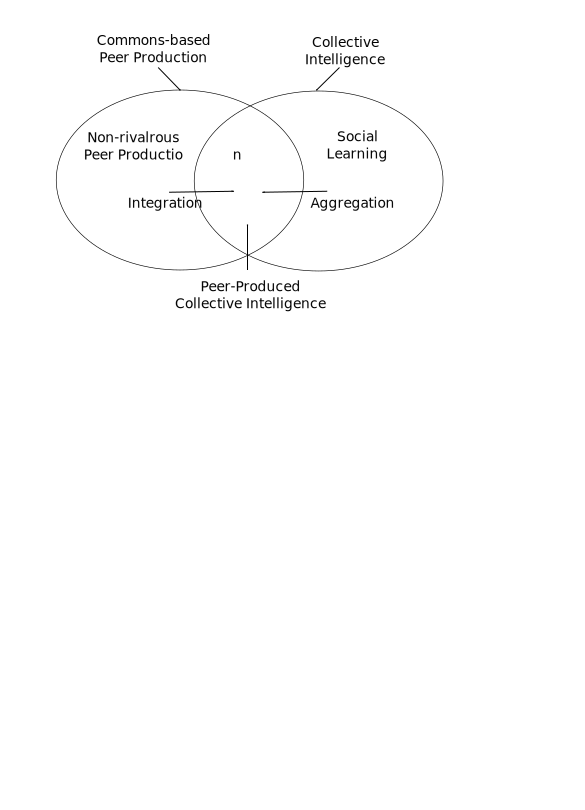
\includegraphics[width=3.75in]{images/fig-peer-intelligence.pdf}
\caption{
Commons-based peer production relies on social learning for
accreditation and integration. Collective intelligence relies on peer
production for ideation and preference aggregation.\label{fig:peer-intelligence}
}
\end{figure}

Benkler (2002) identifies the economic conditions that favor peer production. Specifically, he notes that peering must be more efficient than market-based solutions (Coase, 1937) and that the cost of enforcing contract or property rights must outweigh the benefit (Demsetz, 1974). When do these conditions occur? Benkler attributes the benefits of peer production partly to larger groups having access to more resources, but primarily to allocation gains and information gains. He argues that, with the low cost of communication and storage, creativity is often the scarce resource, and that creative talent is variable and task-specific. The variability of creative work makes it difficult to allocate the right people to the right task. Peer production overcomes this difficulty by letting individuals self-assign. This benefit is amplified in the absence of property rights, which would otherwise limit individuals to working on tasks entirely within one firm. Benkler writes, ``The widely distributed model of information production will better identify who is the best person to produce a specific component of a project, all abilities and availability to work on the specific module within a specific time frame considered." The lack of property rights also allows any combination of collaborators to form a sub-group to work on a sub-task, allowing increased functional diversity, which Hong and Page (2004) have shown is important for teams collaborating to solve difficult problems.

The relative value of peer production also depends on the specifics of the task being performed. Benkler writes, ``peer production is limited not by the total cost or complexity of a project, but by its modularity, granularity, and the cost of integration (2002).'' In Section \ref{sec:network-teams}, I will discuss insights on task complexity from collective intelligence and social learning,
and how they might help inform internet-enabled collective action. Similarly, the cost of integration depends both on organizational networks and on networks of trust relationships. Hierarchical organizations have bottlenecks (i.e., managers and information brokers) who increase the cost of integrating ideas from different parts of the network. Given the need for organizational networks to reflect task structure (Conway, 1968), the more interdependent a task is, the more interdependent the organizational network will need to be. Interdependence creates complexity, raising the cost of integration. This cost can be mitigated in the presence of trust, specifically by the ability to predict the behavior of other members, as reflected by many of Ostrom's (2000) design patterns for self-organized collective action.

\section{Social Choice Theory}
One of the most fundamental challenges of collective action is the need to choose a single course of action when group members are in disagreement. This problem has been addressed by philosophers and mathematicians throughout history, and more recently by social choice theory, a subfield within microeconomics. Social choice theory focuses on the how groups choose between alternatives/candidates/proposals. In this paper, I will use the term ``proposal.''

When members of a group disagree on an issue, one approach is to put it to a vote. In certain contexts, voting can be quite effective. Assuming a binary choice with a correct answer, and decision-makers who independently choose the correct answer with probability $p$, the Condorcet jury theorem (Condorcet, 1785) states that when $p > 1/2$, the probability of the majority choosing correctly approaches 1 as the number of decision-makers grows. While a promising result, the assumptions made by this theorem are somewhat artificial. Many important decisions are ``wicked problems,'' having no single correct answer (Hill, 1982; Anderson, 2006). Also, decision-makers are seldom independent (Hong \& Page, 2009), and rarely homogeneous (Anderson 2006; Hong \& Page 2004). I will return to these criticisms in later sections. A third difficulty forms the central focus of social choice theory: when more than two alternatives exist, there are many conflicting ways to compute a winner.

Simple majority and plurality voting are two straightforward voting methods which can give contradictory results. In plurality voting, the proposal with the most votes wins, even if it does not have a majority. In other words, it is possible for the majority of voters to disapprove of the winner. However, requiring a majority creates its own problems. When there are three proposals and no majority exists, supporters of the two less popular proposals can join together behind one of them allowing it to win, despite another being more highly preferred (Brandt et al., 2012).

More sophisticated approaches consider pairwise contests between proposals. For example, a Condorcet winner is a proposal that receives a majority of votes in pairwise contests against all other proposals (Condorcet, 1785; Brandt et al., 2012). It is difficult to argue against choosing the Condorcet winner, when such an alternative exists, but there is no guarantee that it will. The Condorcet paradox (Condorcet, 1785; Brandt et al., 2012) states that even when individual preferences are transitive, group preferences determined by pairwise contests can be intransitive. For example, if there are three alternatives (Rock, Paper, Scissors) it is possible that, in pairwise votes, Rock beats Scissors, Scissors beats Paper, and Paper beats Rock. In this example, none of the alternatives beat both of their competitors in pairwise votes. Similarly, while any choice between a finite set of proposals can be decomposed into a series of binary choices (i.e., option A or not, option B or not, etc.), such decompositions are path dependent, with the outcome depending on the order in which proposals are considered.

Voting methods can be formalized as {\em social welfare functions} in order to evaluate and compare them systematically (Arrow 1950; Brandt et al., 2012). Each voter $i$'s preferences form a total order $<_i$ over all proposals. Social choice theory typically considers voting systems which depend only on the set of all voter preferences $\{<_i: i \in V\}$. This set is the {\em preference profile} (or just {\em profile}). The purpose of a voting system is to map the profile into a single social preference representing the group. Ties are allowed, but in order to avoid the Condorcet paradox, the social preference must be at least weakly transitive. The resulting social preference is thus represented by a weak order, and the voting system by a social welfare function mapping the profile to the social preference. Similarly, if only the first-place winner is needed, a {\em social choice function} maps each profile into a single winner (or set of winners in the case of a tie).

Using the above formalism, Arrow (1950) demonstrated that any social welfare function will be, in some sense, unfair. Specifically, Arrow's impossibility theorem states that no social welfare function can satisfy all of the the following three fairness criteria:
\begin{description}
\item[Weak Pareto efficiency.]{If A is preferred to B in all individual preferences, then A is preferred to B in the social preference.}
\item[Independence of irrelevant alternatives.]{Changing the position of any C within any individual preference will not change the order of A and B in the social preference.}
\item[No dictator.]{Group preference is not entirely determined by one member of the group.}
\end{description}
Social choice theory has thus focused primarily on identifying desirable properties of voting systems and cataloguing the properties satisfied by various systems.

\subsection{Voting Systems}
Social choice theorists have studied many voting systems (Brandt et al., 2012). I will describe a few which are relevant to this prelim.

\begin{description}
\item[Condorcet method]{(Condorcet, 1785).
A majority vote is conducted for each pair of proposals.
If any proposal wins against all others, it is the winner \.
Such a winner is not guaranteed to exist.}
\item[Dodgson's Method]{(Dodgson, 1876).
An extension of the Condorcet method.
For each proposal, the Dodgson score is the total number of adjacent pairs
in the profile that need to be re-ordered to make that proposal a Condorcet
winner.
If a Condorcet winner exists, its Dodgson score is 0 and it wins.
Calculating the Dodgson winner is NP-hard (Elkind \& Slinko, 2016).}
\item[Borda count.]{(de Borda, 1781). Each proposal receives a score:
the total number of proposals less popular than it over all individuals.
This score is its Borda count, and the proposal with the highest Borda count is
the winner. This winner can be found in polynomial time.}
\item[Copeland rule]{(Copeland, 1781).
Majority votes are held between each pair of proposals.
A proposal's Copeland score is the number of pairwise elections won minus
the number lost. The proposal with the highest score wins.}
\item[Ranked Pairs / Tideman method.]{(Tideman, 1987).
Pairwise majority contests are held.
The results are ranked in order of descending margin. In this order,
the winner of each comparison is placed above the loser in the social
preference, unless doing so would create an intransitive cycle.
The proposal with the highest social welfare value wins.
Tideman can be interpreted as a greedy approximation of minimizing the
dissatisfaction of voters with the social preference,
and can be found in polynomial time (Meskanen \& Nurmi, 2006).}
\end{description}

\subsection{Spatial Models}
A noteworthy class of social welfare functions represents proposals and voter preferences as points in a mathematical space, and are thus called {\em spatial models}. One benefit of this representation is that positions can be compared using mathematically-defined distance measures.

The individual preferences within social choice theory can be compared using several distance measures. These measures can be used to define {\em distance-rationalizable} voting systems, which seek to minimize the winner's distance from some ideal position (Elkind \& Slinko, 2016). For example, Dodgson's method minimizes the distance to a profile with a Condorcet winner.

The Kendall tau metric (Kendall, 1938; Brandt et al., 2012) defines the distance between two total orders (i.e., individual preferences) as the number of pairs for which the two orders disagree.

The Spearman correlation (Spearman, 1904) of two total orders is given by the linear (Pearson) correlation between the lists of rank positions. While Kendall tau takes only order into account, Spearman also takes into account the magnitude of rank difference.

An alternative approach to spatial modeling fixes voter preferences and seeks a dominant strategy for selecting a proposal with the highest chance of winning. Such a model could, for example, represent a political candidate choosing a platform based on their perception of voter preferences and other candidates' positions. In the simplest models, voter preferences are represented as a continuous variable in one dimension (e.g., liberal-conservative). Davis et al. (1970) consider both single-dimensional and multi-dimensional models. For single-peaked preferences in one dimension, the dominant strategy is the position of the median voter. For preferences with more than one peak, it is possible that no dominant strategy exists. For spatial models with multiple peaks or multiple dimensions, the best strategy can exhibit path dependence, depending on which order proposals are defined. Davis et al. also consider the influence of voter abstention on strategy, assuming that alternatives may lose votes to abstention for two reasons. First, voters may abstain if they are {\em indifferent} between two outcomes. Second, voters may abstain if they feel {\em alienated} from the political process and unable to influence the outcome. Under these assumptions, moderate positions can be effective at shifting extreme positions toward the center. It is also possible for an alternative to win over another with higher support if support for the majority position is more dispersed in preference space. In practice, voters' ideal points in preference space are latent but can be inferred from behavioral signals such as past votes (Clinton \& Rivers, 2004).

Returning to the problem of aggregating preferences, the median voter can be useful even in multiple dimensions. The median can be generalized to multiple dimensions as the point which minimizes the sum of distances to all other points. If pairwise distances between voters form a {\em median graph}, then a series of 3-way votes can efficiently find the median (Goel \& Lee, 2012; 2016). Furthermore, the median is either the Condorcet winner (if it exists) or a good approximation. Goel and Lee (2012) propose an efficient method to find an approximation of the generalized median. The Goel-Lee method chooses a triad of 3 voters at random, then asks each to vote between the top preferences of the other two. All three are then required to vote for winning proposal in the next time they vote. The population converges to the generalized median in $O(n \log^2 n)$ triads.

\section{Discourse, Deliberation, and Democracy}
While the paradoxes of social choice theory seem to bode ill for participatory decision-making at large scales, there is more to decision-making than voting. Voter preferences are not fixed, but influenced by public opinion and discourse. The ability to change preference profiles through deliberation suggests the possibility of resolving conflicts prior to the decision-making stage. The ability of the internet to enable discourse and deliberation at a large scale suggests it might make new forms of decision-making, collective intelligence, and therefore collective action, possible. Discourse, deliberation, and voting are distinct but intimately related components of participatory decision-making. Group members share information and opinions through discourse, persuade through deliberation, and aggregate preferences through votes.

\subsection{Democracy}
Democracy is delineated from other forms of collective action by universal participation without the need for actions to be universally supported. It relies on two institutions: votes and talk (Anderson, 2006). Talk includes both the discourse of the public sphere as well as the deliberation of formal and informal bodies. Votes are necessary both to identify winning proposals to give them legitimacy.

In contrast to authoritarian governance, there are several arguments for democracy. Centralization limits the ability of decision-makers to use widely-dispersed information, while democracy enables collective intelligence (Hayek, 1945). Procedural arguments favor democracy as more fair, while epistemic arguments favor it as more effective (Anderson, 2006). Anderson gives three conditions necessary for democracy to be an option: 1. A matter of public interest, 2. Necessity for joint action, and 3. Reliance on the law. Because cooperation is required despite a lack of universal agreement, democracy relies on some level of coercion of dissenting group members through the law.

Talk (discourse and deliberation) plays several roles in democracy. At the ideation and deliberation stages of collective action, the  role of talk is to generate and evaluate ideas. This process consists of discourse within and communication between ``multiple, cross-cutting organizations'' (Anderson, 2006). In ``strong democracy,'' participation is emphasized over voting (Gonz\'alez-Bail\'on, 2010). By doing so, conflict resolution is shifted from coercion of dissenters at the execution stage to building agreement at the deliberation stage. For democracy to function, members do not need to agree with the group's decision, but they do need to cooperate. Dissent, by prompting deliberation, can secure the cooperation of dissenting individuals through ``mutual accommodation'' (Anderson, 2006).

\subsection{Discourse and the Networked Public Sphere}\label{sec:discourse}
As public discourse moves from older broadcast media and onto the internet, its context has changed. Yochai Benkler coined the term networked public sphere (Benkler, 2006) to refer to the unique affordances the internet offers for public discourse, building on sociological concept of the public sphere (Habermas, 1964). The public sphere refers to the social communication conducted by private individuals when they assemble into a public body, for example: newspapers, radio, and television.

The networked public sphere is notable for the affordances offered by the internet: scale, speed, decentralization, and low cost of speech (Benkler, 2002; 2006). The internet operates at a global scale, allows instantaneous publication, is difficult for any single entity to control, and allows the entire public the opportunity to speak without large investments of capital. However, the internet also faces challenges as a medium for pubic discourse, including: fragmentation, emergent centralization, authoritarian filtering, replacing traditional media's role as a watchdog, and the digital divide.

The wide participation enabled by the large scale of the internet also creates the potential for fragmentation of the public sphere into isolated communities (Geiger, 2009; Benkler, 2006). There have been two common solutions for integrating the discourse of very large groups of people online. The first is algorithmic. For example, the Google search engine aggregates data from sources across the internet to gauge the quality of content (Benkler, 2006). However, algorithmic integration is insufficient for creating a public sphere because it is not discursive: running an algorithm is not a social communicative act between humans (Geiger, 2009). The second resolution is the use of technology to enable discursive interactions between large groups, such as reputation systems, peer review, and structured posting privileges (Benkler, 2006).

Discursive integration of peer-produced content depends crucially on the ability of the internet to amplify salient information to a wide audience while filtering out irrelevant information. When the amount of information online is far greater than any one person can sift through, how can this amplication and filtering happen without resorting to non-discursive algorithmic solutions? The answer is again, decentralization. By participating in small topical and organizational groups, individuals have venues to send and receive information relevant to that group and anyone in it. And by participating in multiple such groups, information can quickly spread through the communities where it is relevant. For example, information about a new species of insect might travel from a university email list, to a forum for insect enthusiasts, to a blog for exterminators. This is what Benkler (2006) refers to as a ``filtering and transmission backbone.'' Geiger (2009) describes the process:
``Filtering, accreditation, synthesis, and salience are created through a system of peer review by information affinity groups, topical or interest based. These groups filter the observations and opinions of an enormous range of people and transmit those that pass local peer review to broader groups and ultimately to the polity more broadly." Such systems allow filtering and synthesis through trial-and-error rather than through careful planning; through evolution rather than engineering. Such systems are particularly applicable when errors can recovered from relatively easily.

The structure and protocols of the internet were designed to be decentralized (Baran, 1964), and while necessary for a decentralized sociotechnical system, decentralized architecture and protocols are not sufficient. Centralization can emerge within a decentralized framework due to social, organizational, and economic processes. In fact, the internet exhibits centralization on the levels of router connections and web links (Albert et al., 2000) as well as market share (Noam, 2003). However, this centralization differs from the centralization of traditional media in important ways. Small clusters of sites exceed the activity predicted by power-law distributions (Pennock, 2002). These overlapping topical and organizational clusters create the ``filtering and transmission backbone" (Benkler, 2006). This backbone is bidirectional, allowing utterances from peripheral parts of the network to quickly reach central sites for amplification. This backbone also contains redundant paths not typical of more traditional media, allowing utterances many opportunities for both filtering and amplification. As long as communication is redundant and bidirectional, emergent centralization on the internet is not at odds with public discourse.

The existence of overlapping topical, organizational, and geographic clusters plays an important role in civic participation and discourse (Putnam, 2000; Anderson, 2006; Geiger, 2009), in part by counteracting fragmentation and centralization (Benkler, 2006). When individuals from different clusters interact, there is a potential for a clash of culture and norms. Norris and Inglehart (2009) describe four possible scenarios for cross-cultural communication. In the L.A. effect, a dominant cluster exports its own cluster to others. In the Bangalore effect, cultures from different clusters mix and coexist. In the Taliban effect, conflicting cultures polarize against each other. Finally, in the firewall effect, different cultures simply ignore each other despite the ability to communicate. While the L.A. and Bangalore effects are conducive to a networked public sphere, the others are not. For internet-enabled collective action to be possible on a large scale, technology must conflict resolution through communication, rather than through polarization or isolation.

\subsection{Deliberation}
Deliberation, in contrast to voting, is social communication intended to change the preferences of the participants (Gonz\'alez-Bail\'on et al., 2010). This might occur through social learning (Hill, 1982) or through changes in preferences created by the act of deliberation itself (Anderson, 2006). In other words, deliberation can alter preferences towards actions by altering the predicted outcomes of those actions, or by changing the preferences of the outcomes themselves (Figure 2).

In ``strong democracy'' there is universal participation in deliberation, not just in voting (Gonz\'alez-Bail\'on et al., 2010). Deliberation can be classified on two axes: representation, and argumentation (Figure \ref{fig:deliberation}) (Ackerman \& Fishkin, 2002). An editorial is limited in representation and argumentation. A televised debate is limited in representation, but high on argumentation. A national poll is high on representation but low on argumentation. ``Constitutional moments'' when the population is widely debating a topic fall into the category of high representation and high argumentation, but have traditionally been infrequent and short-lived. Deliberative democracy requires both representation and argumentation, but the two have been difficult to achieve simultaneously, at least with traditional media. Examples of internet-based deliberation, such as Wikipedia (Benkler, 2006) and Slashdot (Gonz\'alez-Bail\'on et al., 2010; Benkler, 2006) have been able to achieve both.

\begin{figure}
\centering
\includegraphics[width=3.75in]{images/fig-deliberation.png}
\caption{Types of deliberation. Adapted from (Ackerman \& Fishkin, 2002).\label{fig:deliberation}}
\end{figure}

Deliberative democracy appeals to procedural arguments for democracy. However, the epistemic merits of deliberative democracy depend on context. Deliberating groups do well on ``eureka problems,'' in which solutions can be easily recognized once they are found, but less well on wicked problems (Gigone \& Hastie, 1997). When groups self-organize into homogeneous groups, deliberation can increase polarization (Schkade et al., 2007) thereby decreasing functional diversity, which is necessary for improved team performance (Hong \& Page 2004). Effective deliberation requires careful attention to both task type and the human tendency towards homophily.

\subsection{Consensus}
There is no consensus on the definition of ``consensus.''
DeTar (2013) classifies several forms of consensus decision-making according to whether they have open membership, egalitarian, formal procedures, binding decisions.

\begin{description}
\item[Corporate (nemawashi).]{Consensus-building informally before formal decision-making. This version can be considered a type of deliberation.}
\item[Scientific.]{A preponderance of agreement among researchers.}
\item[Standards.]{A non-binding agreement between stakeholders.}
\item[Consociationalism / Factional.]{Underrepresented factions are given representation in a formal decision-making body. All formal decisions must be passed by unanimous consent.}
\item[Mob.]{Emergent, unstructured coordination, such as flocking or rioting.}
\item[Assembly.]{Formal body with open membership. All members may or may not have veto power.}
\item[Affinity.]{Small-scale informal decision-making in a closed group. All members have veto power.}
\end{description}

Studies of consensus in social and organizational psychology have typically focused on affinity consensus, categorically excluding formal process (Gentry, 1982). Findings suggest that affinity consensus requires more time than voting, but produces better solutions (Nemiroff \& King, 1975). When trained in the following affinity consensus principles, group members are more likely to generate new, emergent solutions combining the resources of many group members (Hall \& Williams, 1970). 
\begin{itemize}
\item{Avoid arguing for your own position.}
\item{Avoid win-lose stalemates in discussion.}
\item{Avoid changing your mind only in order to avoid conflict and to reach agreement and harmony.}
\item{Avoid conflict-reducing techniques such as majority vote, averaging, bargaining, coin flipping and the like.}
\item{View differences of opinion as both natural and helpful rather than as a hindrance in decision-making.}
\item{View initial agreement as suspect.}
\end{itemize}
These findings suggest that epistemic arguments for democracy based on collective intelligence might better apply to consensus.

While ``consensus'' connotes agreement, many groups using affinity consensus do not require unanimous agreement. Quakers, for instance, use consensus to seek the ``Spirit of God'' and the ``sense of the meeting'' (Gentry, 1982). So consensus implies recognition of the conclusion reached by a group, but not necessarily agreement with that conclusion.

\section{Conflict and Influence}
If deliberation can be used to reduce conflict before decision-making,
it is necessary to understand the social processes of conflict and influence.
In representative democracy, focus is shifted from discourse to voting, 
Enabling scalability at the cost of civic participation and the risk of the Condorcet paradox. Internet-enabled peer production has been able to overcome scaling difficulties while maintaining (or growing) discourse and participation. And as seen in the previous section, conflict can be a sign of functional diversity that enable emergent solutions. But what are the elements of large-scale collective actions that are able to resolve conflict?

The successful resolution of conflict often requires trust and cooperation. In the simple example of the prisoner's dilemma, the dominant strategy for a single round game is to defect rather than cooperate, despite this strategy yielding the outcome with lowest social welfare. However, in an evolutionary model with repeated games, communities can develop norms regarding trust, allowing them to cooperate, resolve conflict, and achieve higher social welfare (Axelrod, 1997a; Ostrom, 2000). In this context, ``a norm exists in a given social setting to the extent that individuals usually act in a certain way and are often punished when seen not to be acting in this way (Axelrod, 1997a).'' Many of Ostrom's design principles for self-organized collective action concern trust and norms, such as clear group boundaries (to identify who the norms apply to) and graduated sanctions (to reinforce norms) (Ostrom, 2000). In addition to norms, communities can exhibit metanorms: norms regarding the enforcement of norms. When metanorms exist to punish individuals for failing to punish transgressions, genetic algorithm simulations suggest that communities can converge to a state where transgressions are rare (Axelrod, 1997a). Internal enforcement, i.e., guilt and shame, also play an important role in influencing behavior. Guilt relies on an internalized sense of allowed behavior, while shame relies on ``social proof'', the visibility of actions to others (Axelrod 1997a).

While dominance hierarchies are not compatible with collective action, there are non-hierarchical forms of dominance which might be. Using ``leveling mechanisms'' such as public opinion, ridicule, and disobedience, some small human societies are effective at ``keeping aggressive and dominating individuals in check'' (Boehm et al., 1993). Leaders in such societies are often described as being ``a first among equals.'' It is not that dominance is non-existent in such societies, it is that it is non-hierarchical. {\em Reverse dominance hierarchies} use dominance to reduce inequality. Similarly, in ``heterarchies'' individuals are simultaneously subordinate and superordinate to many others, enabling the use of dominance for conflict resolution without creating a single hierarchy of power (Sharp, 1958; Tonkinson, 1988; Crumley, 1995).

\section{Social Learning}\label{sec:social-learning}
A crucial part of collective intelligence is the ability of group members to learn from each other. In social learning, individuals receive different information and are each able to communicate with some subset of others. There are many types of social learning, depending on the task being learned, the type of interaction between group members, the network structure of who communicates with whom. Social learning has been extensively modeled both mathematically and using agent-based models.

In the simplest learning problems, agents receive a {\em generated signal} (Hong \& Page, 2009): a measurement of some true value with independent random noise. For example, Galton's ox (Galton, 1907) could be fall into this category if one assumes that errors in guessing are independent and effectively random. The Condorcet jury theorem also falls into this category (Condorcet, 1785). Such problems can be solved by repeated averaging of information with neighbors (DeGroot, 1974). This approach converges to the true value as long as the communication is regular: all individuals have influence on the same number of neighbors (Golub \& Jackson, 2012). When individuals have different influence, the process experiences ``persuasion bias'' and the noise of the most influential individuals is interpreted as signal. The speed of convergence also depends on the communication structure, specifically the second eigenvector of the interaction matrix, which quantifies the existence of bottlenecks in the network (Golub \& Jackson, 2012), with higher connectivity producing faster convergence (Zollman, 2010). In the somewhat more realistic ``bounded confidence'' model, agents average opinions with neighbors only if those opinions differ from their own by less than a ``tolerance parameter'' (according to a spatial model). In this model, moderately tolerant groups benefit from higher connectivity, while low-tolerance groups benefit from central individuals who can act as bridges (Zollman, 2012). While simple social learning tasks such as these are relatively well-understood, they are not particularly good models for real-world problems. Most problems in life are complex.

Complex social learning problems are composed of interdependent sub-problems.
Interdependence results in many locally optimal solutions when sub-problems are
solved in isolation.
There may be more sub-problems than any individual agent can consider.
In this case, agents are in an {\em intepreted signal} regime, and must take a {\em perspective} by focusing on some subset of the full
problem and use {\em heuristics} to make decisions with limited knowledge (Hong \& Page, 2009).

Complex social learning problems can be modeled as optimization problems. Agents search a space of parameters for one that optimizes an objective function. In ``rugged landscapes,'' the objective function has many local maxima, making search by gradient ascent impractical. Such landscapes can be created using the NK model (Kauffman, 1987). In this model, states have N dimensions or loci, with each dimension having a finite number of possible values (e.g., 0 or 1 in the binary case). Associated with each locus is a function $F_i$ depending on that locus and $K$ others. The $F_i$ are randomly assigned values in $[0,1]$ for each possible value of locus $i$ and its $K$ neighbors. An objective function is created by averaging all of the $F_i$. By varying $K$, the ruggedness of the objective function can be tuned.

Agent-based models of complex social learning problems have addressed the role of network structure and social learning strategies in complex problems. Agents can employ a range of behavioral strategies in a social learning setting. In conformity-based strategies (Mason \& Watts, 2012), an agent adopts the solution most popular among its neighbors. In best-neighbor strategies (Lazer \& Friedman, 2007; Grim et al. 2013), an agent evaluates the solutions of their neighbors and adopts the best one. Models exhibit a tradeoff between exploration of new solutions and exploitation of known solutions depending on both network structure (Lazer \& Friedman, 2007) and social learning strategy (Barkoczi \& Galesic, 2016). Such a tradeoff is a characteristic of real-world complex problems (March, 1991). A similar tradeoff exists for performance and efficiency (Platt \& Romero, 2018). Sparsely connected networks result in parallel problem solving and greater functional diversity (Lazer \& Friedman, 2007). Conformity-based strategies also enable greater functional diversity by allowing popular but sub-optimal solutions to persist (Barkoczi \& Galesic, 2016). Combinations of network structure and learning strategy which balance exploration and exploitation yield the best long-term performance (Barkoczi \& Galesic, 2016).

In a real-world setting, the importance of network connectivity can be interpreted as the importance of intersecting and cross-cutting social groups (Anderson, 2006; Benkler 2006; Putnam, 2000). The importance of social learning strategy has implications for the effectiveness of discourse decision-making, which explores many new and existing solutions, versus voting which singles out the best existing solution. However, it is important to note that the social component of collective action is not simply a matter of exchanging information, but also a matter of building trust and mutual accommodation (Anderson, 2006), which are not reflected in current agent-based models.

\section{Networks, Teams, and Tasks}\label{sec:network-teams}
\subsection{Decentralization and Non-hierarchicalism}
The potential benefits of internet-enabled collective action stem largely from allowing groups to grow in size without requiring centralization. ``Decentralization'' has long been a buzzword when discussing the internet, but the term has taken on several distinct meanings. It is necessary to consider precisely in what sense internet-enabled collective action is decentralized and what the affordances of that type of decentralization are.

The internet grew out of research on decentralized communication networks (Baran, 1964). The goal of this early research was to introduce redundancies so that the network could not be disabled by nuclear attacks on central hubs. Baran described three architectures: centralized, decentralized, and distributed (Figure \ref{fig:decentralization}). In Baran's taxonomy, centralized networks have a single central hub that intermediates between all other nodes in the network (for example, the local telephone networks of the time). Decentralized networks are then any network that does not have a single central hub, but might still have a division between endpoints and hubs. In the extreme, distributed networks (e.g., mesh networks) have all nodes play equivalent roles, acting both as end-points and intermediaries. In this taxonomy, decentralized networks exhibit two distinct properties. First, there is more than one intermediary node. Second, endpoints can be connected by multiple redundant paths, passing through different intermediaries. For example, a corporate organizational hierarchy exhibits the first type of centralization, but not the second: middle-managers exist as additional intermediaries, but there is exactly one chain of command from the CEO down to each employee. So it is important to distinguish not just between centralized and decentralized networks, but also between hierarchical and non-hierarchical networks.

\begin{figure}
\centering
\includegraphics[width=4in]{images/fig-decentralized.png}
\caption{
Centralized, decentralized, and distributed network topologies. Adopted from (Baran, 1964).
\label{fig:decentralization}
}
\end{figure}


To further complicate matters, the term ``hierarchy'' is used in multiple ways. Crumley (1995) distinguishes between scalar and control hierarchies. Elements in a scalar hierarchy are composed of sub-components, which are themselves composed of sub-sub-components, and so on (e.g., state, city, address). Control hierarchies on the other hand, involve dominance relationships between components; each relationship is composed of one subordinate and one superordinate element. So the divisions, departments, teams, and individuals of a corporate firm form a scalar hierarchy, while the CEO, regional managers, local managers, and individual contributors form a control hierarchy. It is worth emphasizing that the former is possible without the latter, as in the case of self-managed organizations (Gray et al., 2015) and heterarchies (Crumley, 1995).

The existence of multiple types of decentralization implies that a nuanced approach is necessary to study decentralized collective action. Sociologists and network theorists have developed many techniques for discussing decentralization more precisely. The presence of structural holes in communities allows them to be divided into smaller sub-communities (Burt, 2009; Gonz\'alez-Bail\'on \& Wang, 2016). Those structural holes can in turn be spanned by liaisons/bridges (Rappoport, 1963). Granovetter (1974) proposed that weak ties, individuals with a weak connection and no common friends, play an important role as bridges. He formalized a bridge as a connection that disconnects the entire network if broken, and an n-local bridge as a connection between two nodes whose next shortest connecting path is length n. Liaisons, bridges, and weak-ties have the potential to act as brokers and gatekeepers of information (Gonz\'alez-Bail\'on \& Wang, 2016), a form of social capital (Putnam, 2000). The existence of multiple paths in a decentralized network allows for transmission of conflicting information and attitudes. Balance theory (Rappoport, 1963) suggests that in social networks, when two ties reflect conflicting attitudes, only one will survive, placing constraints on the types of networks that can remain stable.

Focusing on how to achieve non-hierarchical decentralization, DeTar (2013) describes several means:

\begin{description}
\item[Replication.]{Elements are copied and exist independently. For example, the free/open-source Wordpress blogging software can be considered decentralized in the sense that anyone can run a copy independently on their own server.}
\item[Federation.]{In a federated system, such as email or the Mastodon social network, all elements are independent but interoperable. Different email servers can have different owners, run different software, and exist in different locations, but still communicate via a shared protocol.}
\item[Subsidiarity.]{Systems providing different functionality exist independently. For example, embedding a YouTube video on a Wordpress blog that allows users to log in through their Mastodon account.}
\end{description}

The above examples raise another point: decentralization in one domain typically relies on centralization in another (DeTar, 2013; Wilcox-O'Hearn, 2001). For example, the internet's interconnection network is decentralized by relying on a centralized protocol. This centralization/decentralization relationship suggests that some form of centralization is unavoidable. Due to this constraint, Zooko's triangle (Wilcox-O'Hearn, 2001) conjectures that any network protocol can be, at best, two of the following: decentralized, secure, human-readable.

Although less common than centralized, or hierarchical-decentralized organizations, non-hierarchical decentralized regimes can be found in the world today. Elinor Ostrom (2010) has studied several such organizations, including municipal water and police departments, dubbing this type of organization polycentric. In contrast to the assumption that non-hierarchical organization necessarily results in chaos and disorder, Ostrom found that under certain conditions, polycentric governance can take advantage of economies of scale while avoiding diseconomies. She attributed these advantages to three mechanisms: 1. small-to-medium-sized cities are often more effective at monitoring their own performance, 2. citizens who are dissatisfied can vote with their feet by moving into another group, and 3. local incorporated communities can contract with larger producers. Ostrom also noted the role of polycentric governance structure in promoting cooperative behavior. Rational choice models, often used to explain non-cooperation, do not take communication or individual agency into account. As such, Ostrom proposes the following conditions for cooperation within polycentric governance:
\begin{enumerate}
\item{Communication feasible with all participants,}
\item{Reputations are known,}
\item{High marginal per capita return,}
\item{Ability to enter/exit,}
\item{Longer time horizon,}
\item{Agreed-upon sanctioning.}
\end{enumerate}

Based on observations of polycentric governance regimes, Ostrom summarizes: "complexity is not the same as chaos in regard to metropolitan governance." In this prelim, I investigate some of the questions necessary to extend Ostrom's observation to internet-enabled collective action.

\subsection{Task Structure}
While social network structure is well-studied, the structure of tasks themselves is less well studied. It may not be obvious that tasks can have structure or what that means. As in social learning, one dimension of task structure is interdependence: how effectively can sub-parts of a problem be solved independently? Low-interdependence and task granularity, are key component of commons-based peer production (Benkler, 2002; Kittur \& Kraut, 2008). The granularity of a problem relative to the number of problem solvers also influences whether it is best modeled as a generated signal or interpreted signal problem (Hong \& Page, 2009). When a problem can be considered on many dimensions, problem solvers are more likely to focus on different subsets up the problem, as in interpreted signal problems.

Centola and Macy (2007) discussed how the role of network structure is modulated by task structure. They distinguish between simple contagion (information diffusion) and complex contagion. In the former, only a single exposure is necessary for information to propagate, while in the later, multiple exposures are necessary. Such might be the case when individuals are looking to others for social signals about the relative risk or safety of adopting an innovation. They note that long ties are unable to spread complex contagions, despite their effectiveness at propagating information such as job opportunities (Granovetter, 1974).

In the organizational psychology literature, Hill (1982) identifies several classes of group tasks:

\begin{description}
\item[Learning]{Examples include: memorization, concept-attainment/classification.}
\item[Mastery/creativity.]{Examples include: learning the meaning of words and identifying synonyms/antonyms.}
\item[Abstract problem solving.]{Examples include: completing partially written poems, finding efficient travel routes connecting multiple points.}
\item[Brainstorming.]{Examples include: thinking of proposals to ensure schools perform well as enrollment increases.}
\item[Complex problem solving.]{Examples include: a manager incorporating conflicting suggestions on ways to improve the work process.}
\end{description}

These task structures appear to have implications for how groups collaborate. In any analysis of collective action, and in the design of internet-based tools for collective action, it will be necessary to be aware of the nature of the task being approached and how it differs from any existing examples.

\subsection{Organizational Networks}
Organizations and firms with formally defined roles and relationships provide a context in which network structure is at least partially visible and can be deliberately manipulated. One particularly interesting observation regarding organizational networks is Conway's law (Conway, 1968) which says that the organizational structure of complex systems reflects the social structure of the organization that built them (Figure \ref{fig:conway}). This observation stems from the fact that when sub-tasks are assigned to groups, groups that are disconnected from each other will not be able to solve sub-tasks that are highly interdependent. In Conway's words, ``Given any design team organization, there is a class of design alternatives which cannot be effectively pursued by such an organization because the necessary communication paths do not exist.'' For collective action, the implication is that large interdependent problems are not solvable without a way for large groups to coordinate and cooperate.

\begin{figure}
\centering
\includegraphics[width=3.25in]{images/fig-conway.png}
\caption{
Conway's law: ``There is a very close relationship between the structure of a system and the structure of the organization that designed it.'' Adapted from (Conway, 1968).
\label{fig:conway}
}
\end{figure}

This prelim is largely concerned with the potential for non-hierarchical, decentralized collaboration enabled by the internet, but this should absolutely not be confused with structurelessness. In a classic essay, feminist scholar Jo Freeman wrote about the dangers of (apparent) structurelessness (Freeman, 1972). Freeman argues that all groups have structure, whether it is formal or hidden. Hidden structure can be used to mask power and make participation closed to the greater group, both of which can limit the ability of groups to take full advantage of their resources. Regarding the scaling of communication requirements with group size, Freeman writes, ``This inevitably limits group participants to about five, or excludes some from some of the decisions. Successful groups can be as large as 10 or 15, but only when they are in fact composed of several smaller subgroups which perform specific parts of the task, and whose members overlap with each other so that knowledge of what the different subgroups are doing can be passed around easily.'' While Freeman seems to make the common assumption that structure implies control hierarchy, I argue in this prelim that through concepts like heterarchy (Crumley, 1995), explicit structure can exist in large-scale, non-hierarchical, decentralized collective action.

\subsection{Team Composition}
The success of teams can also be influenced by the personal characteristics of the team members. The Diversity Trumps Ability theorem (Hong \& Page, 2004) describes the conditions under which a diverse group of individuals can outperform a homogeneous group of higher-performing individuals. Specifically: 1. agents must be intelligent, 2. the problem must be difficult such that no individual can solve it on their own, 3. the agents must be diverse, and 4. the best agent must be unique. Hong and Page also used an agent-based model to verify that a random sample of agents can outperform a team of the best agents. The social dynamics of teams must also be taken into account. Hill (1982) noted that interactions between team members were influenced by social roles such as gender. Finally, levels of inequality can influence a team's ability to work together. Nishi et al. (2005) found that when simulated wealth levels were visible in a prisoner's dilemma game, participants wealthy participants took advantage of the less wealthy, leading to a rich-get-richer dynamic, lowering both cooperation and overall group performance. Team success is influenced by many individual characteristics of the team members, and even by the visibility of those characteristics.


